\documentclass[a4paper,12pt]{article}
\usepackage{anysize}
\marginsize{3cm}{3cm}{1cm}{3cm}
\usepackage{amsmath}
\usepackage{amsthm}
\usepackage{bbm}
\usepackage{graphicx}

\begin{document}
\title{\textbf{Computational Statistics: Homework 4}}
\author{Michal Porvaznik \\ Nemesis key = 8676cc2}
\date{March 24, 2015}
\maketitle
%
\section*{Exercise 1}
%
a) Bellow are the autocorrelation plots of the \textbf{bmw} dataset as well as of the squared values. For most lags the autocorrelation of the original data is within the 5\% acceptance region of for testing the null hypothesis of uncorrelated data. This is however not true for the transformed values.
\\
\\
\\
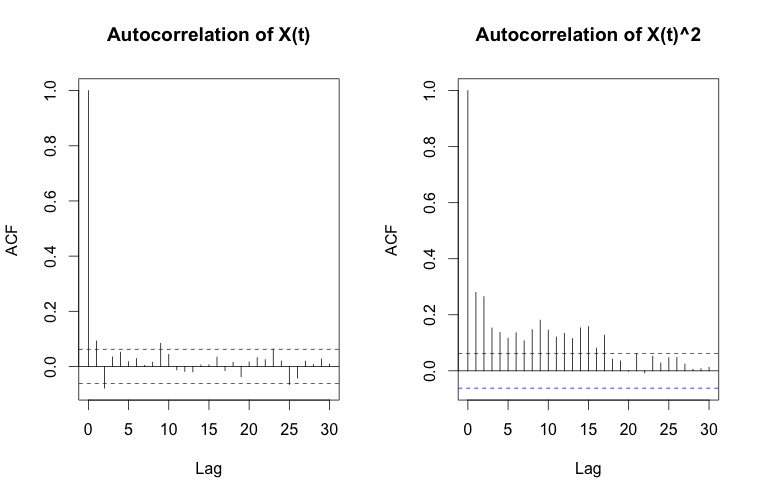
\includegraphics[scale = 0.55]{hmw4_plot1.png}
\pagebreak

b) Below we see the plot of $Y_t = X_t^2 =  v(X_{t-1}) + \eta_t$ for the observed values.

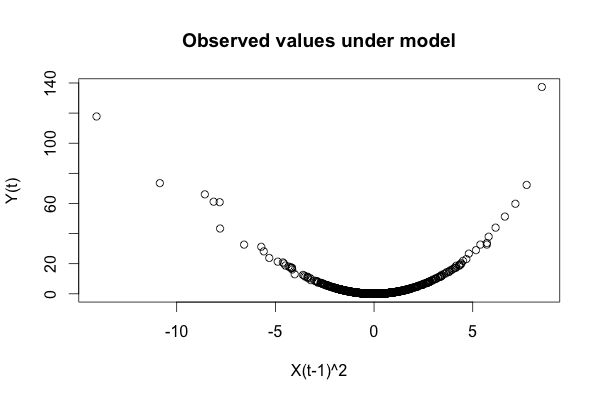
\includegraphics[scale = 0.65]{hmw4_plot11.png}

Upon fitting the three models to the data I obtained the estimate and residual plots bellow. These show that the expected noise is not zero and there the errors are heavily correlated. However, I am not sure what to deduce from this. Does this mean that we should not model the data set using regression?
\\
\\

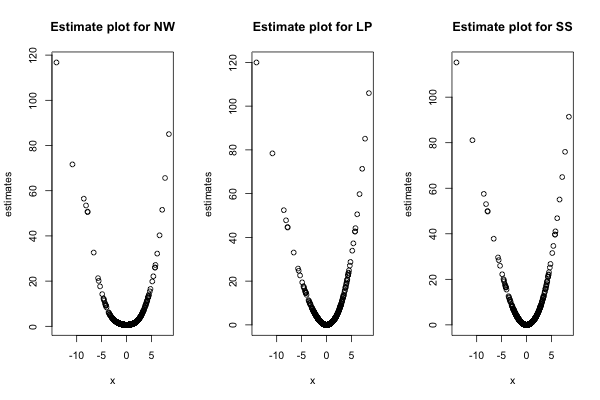
\includegraphics[scale = 0.7]{hmw4_plot21.png}
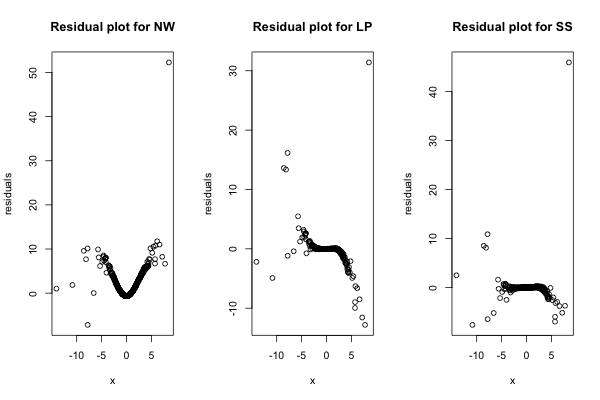
\includegraphics[scale = 0.7]{hmw4_plot2.png}

c) Plots below show estimates and residuals of \textbf{lokern} and \textbf{glkern} fits. In both cases the estimate is good around the center, where we have a lot of observations, but fluctuates closer to boundaries where the observations are sparse. These estimates are so similar that the difference if not even visible on the plots.

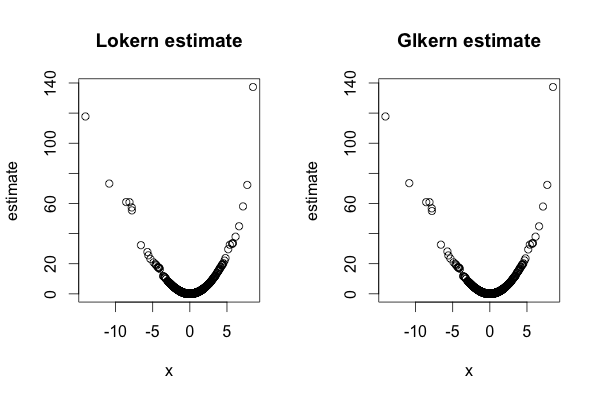
\includegraphics[scale = 0.7]{hmw4_plot4.png}
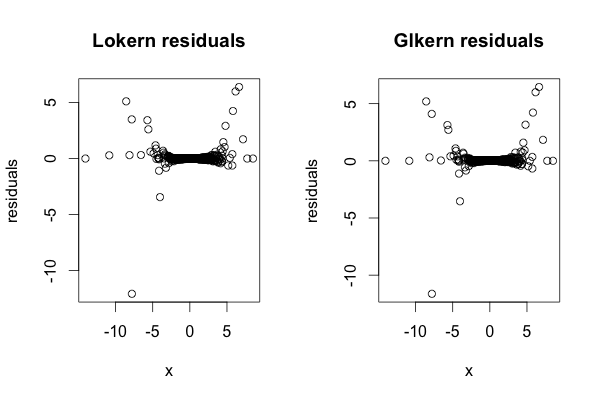
\includegraphics[scale = 0.6]{hmw4_plot5.png}

Here we see the log of local and global bandwidth plots. As expected, the local bandwidth is much smaller where data is dense, but as we can see from the \textbf{rug(x)} the bandwidth is not decreasing strictly with the density. Here again I do not understand why the local bandwidth peaks locally at 0 or why does it even vary. The optimal bandwidth that \textbf{lokern} implements is

\begin{equation}
h_{opt}(x) = n^{-1/5}\Bigg( \frac{\sigma_\epsilon^2 \int{K^2(z)dz}}{\big( m^{''}(x)\int{z^2K(z)dz} \big)^2} \Bigg)
\end{equation}

and I don't see which term of this expression influences the value of the bandwidth, since $m^{''}(x)$ is constant in this case.


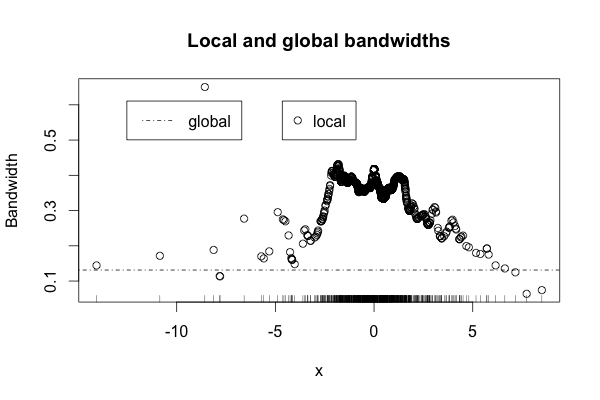
\includegraphics[scale = 0.65]{hmw4_plot6.png}

\end{document}

